\documentclass[edipack2.tex]{subfiles}
\begin{document}

\section{Examples}\label{SecExamples}
In this section we illustrate the functioning of the \NAME
library and their interfaces through specific examples, including
discussion of relevant code snippets.
Specifically, we show how the quantum impurity solver in \NAME can be used
to address problems of different nature within the framework of DMFT. 


\subsection{Bethe lattice DMFT}\label{SecExamplesBetheDMFT}
The description of the Mott or metal to insulator transition (MIT)
within the Bethe lattice, i.e. Cayley tree with connection
$z\to\infty$ is conventionally considered the test bed of any DMFT
application. Here  we discuss a guided implementation based on the
Fortran API of \NAME of the DMFT solution of the Bethe lattice at
$T=0$. 
We consider a Fermi-Hubbard model:
$$
H = -t \sum_{\langle ij\rangle\s}c^+_{i\s}c_{j\s} + U \sum_i n_{i\up}n_{i\dw}
$$
where $c^+_{i\s}$ ($c_{i\s}$) is the creation (destruction) operator for an electron at site $i$
and with spin $\s$, $n_{i\s}=c^+_{i\s}c_{i\s}$ is the occupation
operator and the first sum is over the nearest neighbor sites $\langle
ij\rangle$. 
The system is defined on a Bethe lattice with density of states
$\rho(\e)=\frac{1}{2D}\sqrt{D^2-\e^2}$, where $D=2t$ is the
half-bandwidth~\cite{Georges1996}.
In DMFT this model is mapped
onto a quantum impurity problem with an effective electronic bath
which needs to be determined self-consistently.
\begin{lstlisting}[style=fstyle,numbers=none,basicstyle={\scriptsize\ttfamily}]
program ed_hm_bethe
   USE EDIPACK2
   USE SCIFOR
   implicit none
   !> Number of discretization points for the Bethe DOS
   integer,parameter                           :: Le=5000
   !> Bethe half-bandwidth = energy unit
   real(8),parameter                           :: D=1d0
   !>Bath:
   real(8),allocatable                         :: Bath(:)
   !> local dynamical functions, rank-5 [Nspin,Nspin,Norb,Norb,L]
   complex(8),allocatable,dimension(:,:,:,:,:) :: Weiss,Smats,Sreal,Gmats,Greal,Weiss_
   ... (omissis)
   !> READ THE input using EDIpack procedure:
   call ed_read_input(trim(finput))
   !
   !> Setup the Bethe DOS $\rho$ (linear dispersion)
   Ene = linspace(-D,D,Le,mesh=de)
   DOS = dens_bethe(Ene,D)
\end{lstlisting}

The bath is described
by the (unknown) function $\GG^{-1}_0$, i.e. the Weiss field. Within \NAME
exact diagonalization approach, where the bath is approximated with a
finite number of levels, the function $\GG^{-1}_0$ is used to
determine bath parameters $\vec{x}=\{V,h\}$ using the optimization method discussed in
\secu{sSecFit}.
The starting point of any calculation is determined by a suitable
guess of the Weiss field, or equivalently of the bath parameters.
In \NAME this operations is accomplished by the function {\tt
  ed\_init\_solver}.

\begin{lstlisting}[style=fstyle,numbers=none,basicstyle={\scriptsize\ttfamily}]
Nb=ed_get_bath_dimension()
allocate(bath(Nb))
call ed_init_solver(bath)
\end{lstlisting}








The iterative algorithm proceeds as follows:
\begin{enumerate}
\item Call the exact diagonalization {\bf impurity solver} {\tt
    ed\_solve} whose only input is the set of parameters $\vec{x}$. All other
  options are controlled by input file specifications ({\tt
    ed\_read\_input}).
\item Retrieve at least the self-energy functions $\Sigma_{\a\b\s\s'}(i\omega)$ on the
  Matsubara axis using {\tt ed\_get\_sigma}.
\item Evaluate the local interacting Green's function
  $G_{loc}(i\omega) = \int_{-D}^D \frac{\rho(\e)}{\zeta -\e}d\e$ with
  $\zeta=i\omega+\mu-h^0-\Sigma(i\omega)$.
  \item Update the Weiss field through the {\bf self-consistency}
    relation: $\GG^{-1}_0(i\omega) = G_{loc}(i\omega) + \Sigma(i\omega)$. 
  \item Optimize the bath parameters $\vec{x}$ against the updated
    Weiss field using, for instance, {\tt ed\_chi2\_fitgf}. Restart at 1.
\end{enumerate}
In agreement with Reverse Communication Strategy setup, the step 3-4
are left to the user. In addition step 5 is kept separated to
guarantee enough freedom in the bath optimization, though we remark
this is a crucial step which can potentially compromise the whole
calculation.
An example of implementation is given in the following listings.

\begin{lstlisting}[style=fstyle,numbers=none,basicstyle={\scriptsize\ttfamily}]
iloop=0;converged=.false.
   do while(.not.converged.AND.iloop<nloop)
     iloop=iloop+1     
     !> Solve the effective impurity problem
     call ed_solve(bath)     
     !> Retrieve impurity Self-energy on Matsubara axis
     call ed_get_sigma(Smats,'m')
     !
     !> Build a local Green's function:
     wfreq = pi/beta*(2*arange(1,Lmats)-1)   !automatic Fortran allocation
     do i=1,Lmats ! One can do better than this of course 
        zeta= xi*wfreq(i)+xmu - Smats(1,1,1,1,i)
        Gmats(1,1,1,1,i) = sum(DOS(:)/( zeta-Ene(:) ))*de  
     enddo
     !> Update Weiss field: Self-consistency
     Weiss(1,1,1,1,:) = one/(one/Gmats(1,1,1,1,:) + Smats(1,1,1,1,:))
     !> Close the self-consistency fitting the new bath:
     call ed_chi2_fitgf(Weiss,bath,ispin=1)     
     !>Check convergence
     converged =( sum(abs(Weiss(1,1,1,1,:)-Weiss_(1,1,1,1,:)))/sum(abs(Weiss(1,1,1,1,:))) )<dmft_error
     Weiss_=Weiss     
   enddo
\end{lstlisting}


\paragraph{Results}
In the following we present some results obtained for the model
introduced above. Specifically we focus on the testbed case of the interaction
driven Mott transition, descriving the progressive
transformation of a partially-filled band metallic state into a correlated insulator. 

To illustrate this point, we report in panel (A) the evolution of
the spectral function $-{\rm Im}G_{loc}(\omega)/\pi$ as a function of
the interaction strenght $U$. Despite the {\it spiky} nature of the spectrum, due to the
finite size (i.e. number of poles) of the discretized effective bath,
it is possible to clearly distinguish the characteristic features of
the Mott transition. At low energy, we observe the renormalization of the 
quasi-particle peak at the Fermi level ($\omega=0$). Concomitantly the
system shows the formation of incoherent  high-energy features which
will then develop into Hubbard bands in the Mott insulating state for $U>U_c$, with $U_c\simeq 2.8D$. 


\begin{figure}[t!]
  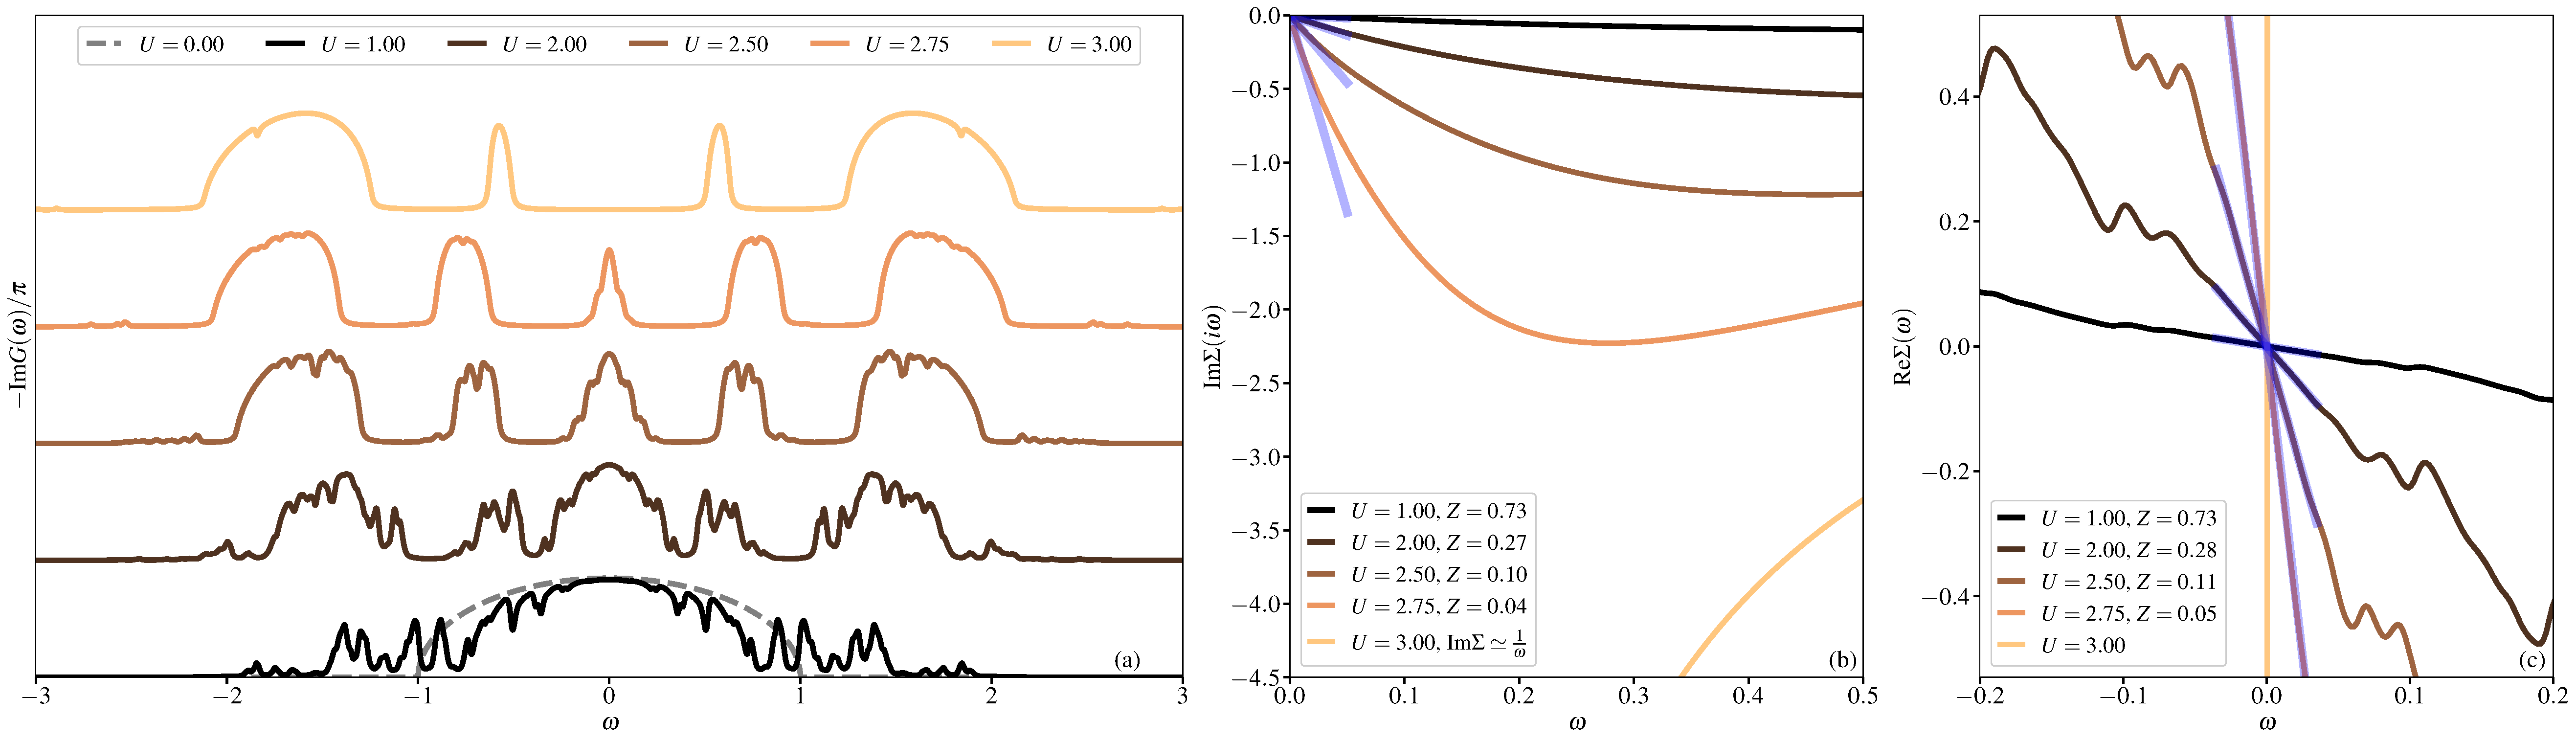
\includegraphics[width=\linewidth]{figures/figBethe.pdf}
    \caption{\label{figEx1}%
      \textbf{The Metal-Insulator Mott transition.}
      (a) Evolution of the spectral function $-\Im{G}(\omega)/\pi$ as
      a function of increasing interaction $U$. The critical
      interaction $U_c\simeq 2.8D$ separates the correlated metal $U<U_c$ from
      the Mott insulator $U>U_c$.
      (b)-(c) The corresponding evolution of the Matsubara self-energy
      $\Im\Sigma(i\omega)$ (b) and
      real-axis one $\Re\Sigma(\omega)$ across the Mott
      transition. For a particle-hole symmetric case both allow to
      estimate the renormalization constant $Z$ (see main text), using
      linear order expansion in frequency (blue solid lines). The
      values of $Z$ are reported in the legend.
      The Mott insulating solution is associated to a singularity at
      $\omega=0$ of $\Im\Sigma$. 
        }
\end{figure}

The formation of a spectral gap separating the Hubbard bands in the
Mott insulator is supported by the divergence, at the Fermi level, of the imaginary part of
the self-energy function. Causality imposes that the real-part of
this quantity becomes large near the singularity making it impossible
to satisfy the quasi-particles poles equations
$\omega+\mu-h^0-\e-\Re{\Sigma}(\omega)=0$, i.e. preventing coherent
quasi-particles excitations near the Fermi level. 
In the panels (B) and (C) we discuss this point  showing the evolution
of the self-energy functions $\Sigma$.
Specifically, in panel (B) we report the self-energy ${\rm Im}\Sigma(i\omega)$
on the Matsubara axis in the low energy regime. Increasing $U$
we observe the progressive growth of this function until a
diverging behavior is acheived crossing the critical interaction
strenght $U>U_c$.
We recall that this behavior can be observed on the Matsubara axis
because of the particle-hole symmetry of the problem which pins the
$\Im{\Sigma}$ singularity at $\omega=0$.
In panel (C), we report the corresponding behavior of the
$\Re{\Sigma}(\omega)$ in small energy regime around the Fermi
level. Augmenting the interaction strength $U$ leads to a sudden
increase of this self-energy component until a discontinuous behavior
is reached, associated to the divergence of the corresponding
imaginary part.   

A quantitative description of the transition is obtained from the
quasi-particle renormalization constant $Z$, which correlates with the degree of
localization of the electrons being equal to 1 for a non-interacting
metal and 0 for the Mott insulator. This quantity is obtained from the
linear term in the Fermi liquid expansion of the self-energy as
$Z=(1-\tfrac{\partial\Re\Sigma}{\partial\omega}_{|_{\omega\rightarrow
    0}})^{-1}$.
Using the relation:
$$
   \frac{\Im\Sigma(i\omega_n)}{\omega_n}_{|_{\omega_n\rightarrow 0}}=
   \frac{1}{\pi}\int_{\mathbb R}d\epsilon \frac{\Re\Sigma(\epsilon)}{\epsilon^2}=
   \frac{\partial\Re\Sigma}{\partial\omega}_{|_{\omega\rightarrow 0}}.
$$
we can extract $Z$ also from the linear behavior of ${\rm Im}\Sigma(i\omega)$ for 
$\omega\to0$ in the metallic regime.

The linear fit highlighted in the panels (B)-(C) and the corresponding values of $Z$ are reported in the legend.
In both cases we observe that increasing $U$ the slope of the linear behavior of the
self-energy at low-energy increases upon increasing $U$, either on the
Matsubara or real-axis. At the transition point the slope becomes
infinite according to the divergence of the imaginary part of
the self-energy  ${\rm Im}\Sigma(\omega) \rightarrow -\infty$,
corresponding to $Z\to 0$. 


\subsection{Attractive Hubbard model (Python API)}\label{SecExamplesAHM}
The second application has the twofold aim to demonstrate the
superconductivity support of the \NAME library as well as to
illustrate the use of the Python API through a working example.
We consider the simple, yet non-trivial, case of the attractive
Hubbard model on a two-dimensional square lattice:

$$
H = \sum_{\ka\s} \e(\ka)c^+_{\ka\s}c_{\ka\s} -U\sum_i n_{i\up}n_{i\dw}
$$
where $U>0$, $c^+_{\ka\s}=\tfrac{1}{\sqrt{N}}\sum_i e^{-i\ka\cdot R_i} c^+_{i\s}$
and $c^+_{i\s}$ is the creation operator for an electron at site $i$
and with spin $\s$, $n_{i\s}=c^+_{i\s}c_{i\s}$ is the occupation
operator and $\e(\ka)=-2t[\cos{(k_x a)}+ \cos{(k_y a)}]$ is the
energy dispersion relation. In the following we the lattice distance
$a=1$  and the energy unit as $4t=D=1$.

The DMFT workflow for this case is very similar to the previous one
provided works in the Nambu basis defined by the spinor
$\psi_i=[c_{i\up}, c^+_{i\dw}]^t$.
In this basis any correlation functions, e.g. the Green's function, takes the matrix form:
\begin{equation}
  {\mathbf G} =
  \begin{pmatrix}
    \hat{G}_{\uparrow\uparrow} & \hat{F}_{\uparrow\downarrow}\\
    \hat{\bar{F}}_{\downarrow\uparrow}  &    \hat{\bar{G}}_{\downarrow\downarrow} \\
   \end{pmatrix}
\end{equation}
where the symbol $\hat{A}$ indicates the possible multi-orbital
character which reduced to a scalar in the present case of a single
orbital. The symbol $\hat{\bar{A}}$ indicates that the components in
the second row are connect by particle-hole and time-reversal
symmetries to the first row one. The specific relation depends on the
symmetry of the order parameter (here $s$-wave) and the nature of the
complex argument of the functions, i.e. Matsubara or real-axis:
\begin{equation}
\begin{array}{cc}
  \hat{\bar{G}}(i\omega) = -\hat{G}^*(i\omega)\;; &  \hat{\bar{F}}(i\omega) = \hat{F}(i\omega)\\
  \hat{\bar{G}}(\omega)  = -\hat{G}^*(-\omega) \;; & \hat{\bar{F}}(\omega) = \hat{F}^*(i\omega)\\
\end{array}
\end{equation}  
The code implementation closely follows the previous structure, with
some notable exceptions related to the Nambu structure for which,
using the symmetries above, we only need to deal with the first row
independent components. In the first part of the code we initialize
the lattice structure and the solver:
\begin{lstlisting}[style=mypython,numbers=none,basicstyle={\scriptsize\ttfamily}]
import numpy as np
from edipy2 import global_env as ed
import mpi4py
from mpi4py import MPI
import os,sys
from aux_funx import * #include function to build $G_{loc}$ and Weiss fields

comm = MPI.COMM_WORLD
rank = comm.Get_rank()
master = (rank==0)

#Functions
def generate_kgrid(Nk):
    b1=2*np.pi*np.array([1.0,0.0])
    b2=2*np.pi*np.array([0.0,1.0])
    n1, n2 = np.meshgrid(np.arange(Nk), np.arange(Nk))
    n1=n1/Nk;n2=n2/Nk
    gridout = np.stack([n1.ravel(), n2.ravel()], axis=-1)
    return np.dot(gridout,[b1,b2])

def h_square2d(k,t):
  return -2*t*(np.cos(k[...,0,np.newaxis,np.newaxis])+np.cos(k[...,1,np.newaxis,np.newaxis]))*np.eye(ed.Norb)
    

ed.read_input("inputAHM.conf")

kgrid = generate_kgrid(Nk)

#Generate hk and hloc
Hk   = h_square2d(kgrid,t_hop)
HkNambu   = np.array([h_square2d(kgrid,t_hop),-np.conj(h_square2d(-kgrid,t_hop))])
Hloc = np.sum(Hk,axis=0)/Nk**2
Hloc = Hloc.astype(complex)
ed.set_hloc(Hloc)

#SETUP SOLVER
Nb=ed.get_bath_dimension()
bath = ed.init_solver()
bath_prev = np.copy(bath)
\end{lstlisting}




The iterative scheme for the solution of DMFT closely follows the
sequence discussed in \secu{SecExamplesBetheDMFT}:   
\begin{enumerate}
\item Call the exact diagonalization {\bf impurity solver} {\tt
    ed.solve} providing the set of bath parameters $\vec{x}=\{V,h\}$  as input. 
\item Using the dedicated
  input/output procedures {\tt ed.get\_sigma} we retrieve the self-energy functions  
  $\hat{\Sigma}(i\omega)$ and $\hat{S}(i\omega)$ on the 
  Matsubara axis.
\item
  Evaluate the interacting local Green's functions $\hat{G}_{loc}$ and
  $\hat{F}_{loc}$:
  \begin{equation}
  {\mathbf G}_{loc}(i\omega) =
  \int_\RRR d\e \rho(\e)
  \begin{pmatrix}
    (i\omega +\mu)\hat{\11} - \hat{h}^0 - \hat{\Sigma}(i\omega) -\e & -\hat{S}(i\omega) \\
    -\hat{S}(i\omega) & (i\omega +\mu)\hat{\11} + \hat{h}^0 +
    \hat{\Sigma}^*(i\omega) +\e\\
  \end{pmatrix}^{-1}
\end{equation}
\item Update the normal and anomalous Weiss fields, respectively 
  $\GG_0^{-1}$ and $\FF_0^{-1}$, through the {\bf self-con\-sis\-ten\-cy}
    relation: $\mathbfcal{G}^{-1}_0(i\omega) = {\mathbf G}_{loc}(i\omega) +
    {\mathbf \Sigma}(i\omega)$ in Nambu space. 
  \item Optimize the bath parameters $\vec{x}$ to best describe the  updated
    Weiss fields using \NAME provided conjugate gradient  fit
    procedure {\tt ed.chi2\_fitgf}.
\end{enumerate}
which is implemented in Python as follows:
\begin{lstlisting}[style=mypython,numbers=none,basicstyle={\scriptsize\ttfamily}]
#DMFT CYCLE
converged=False;iloop=0
while (not converged and iloop<ed.Nloop ):
iloop=iloop+1

    #Solve impurity problem
    ed.solve(bath)
    
    #Self-consistency with aux_funx procedures:
    Smats = np.array([ed.get_sigma(axis="m",typ="n"),ed.get_sigma(axis="m",typ="a")])    
    Gmats = get_gloc(wm*1j       ,ed.xmu,HkNambu,Smats,axis="m") 
    Weiss = dmft_weiss_field(Gmats,Smats)                  
          
    #Fit
    bath = ed.chi2_fitgf(Weiss[0],Weiss[1],bath)

    #Error check
    err,converged=ed.check_convergence(Weiss,ed.dmft_error)

ed.finalize_solver()
\end{lstlisting}


\begin{figure}[t!]
  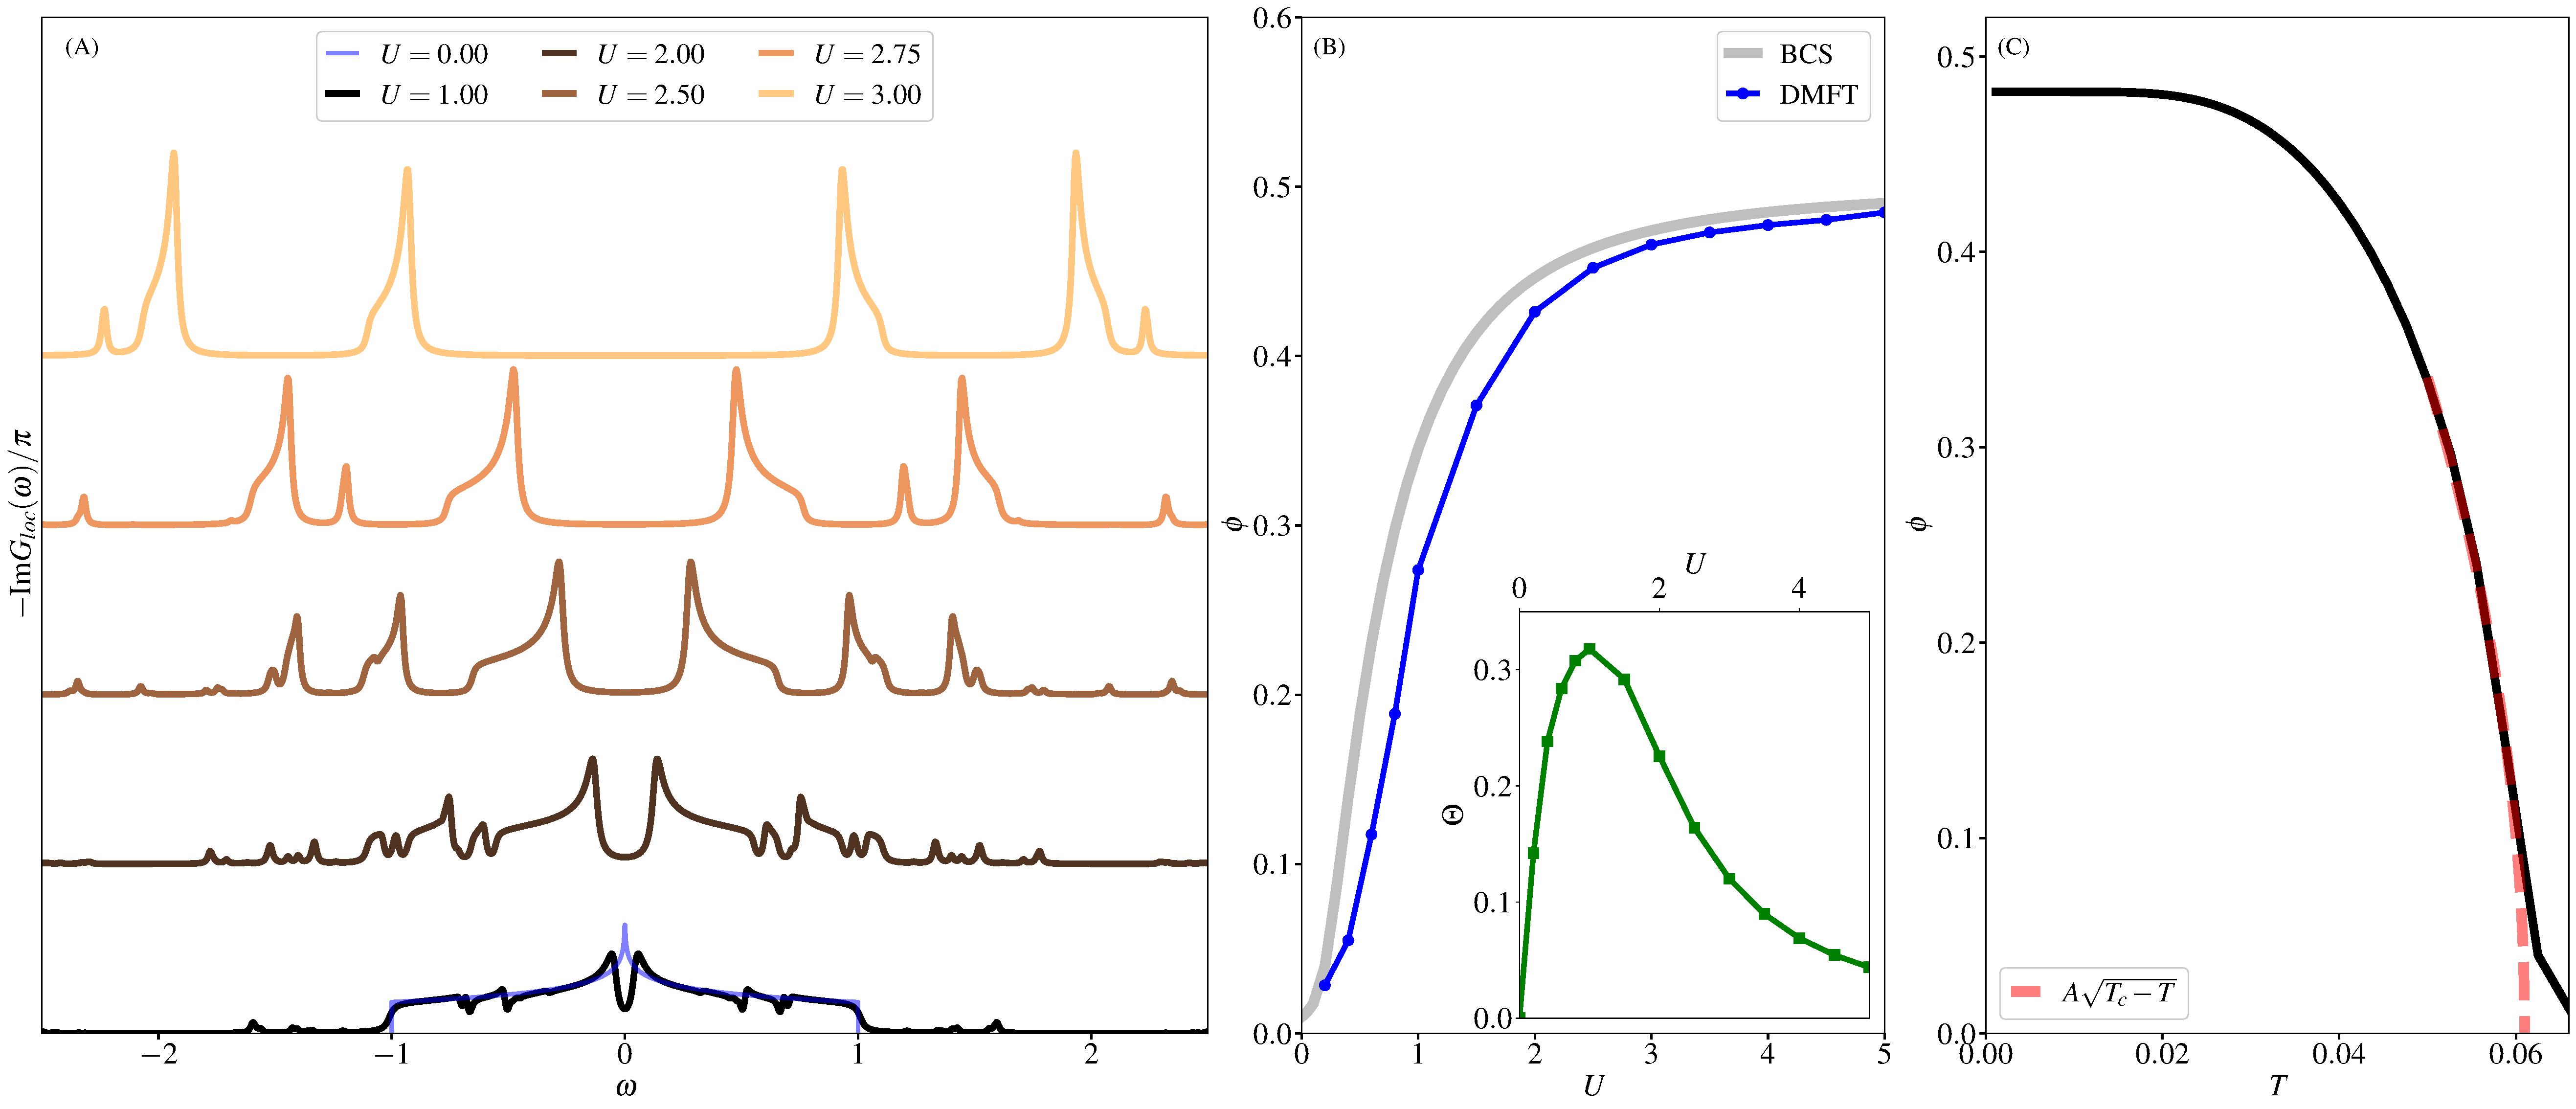
\includegraphics[width=\linewidth]{figures/figAHM.pdf}
    \caption{\label{figEx2}%
      \textbf{The BCS to BEC crossover.}
      (a) Evolution of the spectral functions
      $-\Im{G_{loc}(\omega)}/\pi$ as a function of increasing
      attraction $U$. 
      (b) The order parameter $\phi=\langle c_\up c_\dw\rangle$ as a
      function of the attraction $U$. Data for BCS (gray) is compared
      to DMFT results (blue line and symbols). 
      (c) The correlation strength
      $\Theta=\frac{|S(i\omega\to0)-S(i\omega\to\infty)|}{S(i\omega\to\infty)}$ as a function of the
      attraction $U$ across the BCS-BEC crossover. 
      (d) Comparison of the double occupation $D=\langle n_\up
      n_\dw\rangle$ as a function of attraction $U$ between BCS (gray
      solid line) and DMFT (blue solid line and symbols). 
      (e) Superconducting order
      parameter $\phi$ as a function of temperature across the
      superconductor-to-normal phase transition. Data for $U=4$. The
      fit highlights the critical behavior with a mean-field exponent
      $\beta=1/2$ (red dashed line) and parameters $A\simeq 3.7$, $T_c=0.61$.       
        }
\end{figure}

\paragraph{Results}
We showcase here some results for the DMFT solution of the attractive
Hubbard model across the BCS to BEC regime, with the aim of
illustrating the capabilities of \NAME to deal with $s$-wave
superconductivity at zero and finite temperatures.

To beging with, we report in  panel (A) of \figu{figEx2} the
evolution of the spectral density, obtained from the local normal
Green's function $-\tfrac{1}{\pi}\Im{G}_{loc}(\omega)$, as a function
of the attraction $U$. For any finite value of  $U$ the Van Hove peak
at $\omega=0$ of the 2D square lattice (see $U=0$
solution) gets split by the formation of a superconductive gap of
width which increases with $U$.
The existence of a gap is associated to the formation of a finite
order parameter $\phi=\langle c_\up c_\dw\rangle$. The behavior of
this quantity, shown in panel (B), highlights crossover from the BCS
regime at weak coupling to a BEC one for large $U$.
The former regime is characterized by the well known exponential increase of
$\phi$, which is computationally the hardest regime to adress. At
strong coupling or BEC regime the order parameter saturates to its
limiting value $\phi\to 1/2$. The comparison with mean-field result
(gray) underlines the effect of local quantum fluctuations in slightly
suppressing the order parameter. This effect is particularly active in
the intermediate regime, as captured by the behavior of the
correlation strength
$\theta=\frac{|S(i\omega\to 0)-S(i\omega\to\infty)|}{S(i\omega\to\infty)}$
reported in panel (C). Assuming a monotonic behavior of the anomalous
self-energy function, this quantity estimates the ``strength'' of
quantum fluctuations comparing the mean-field-like behavior at high
energy scale with that near the Fermi level. A large value of $\theta$
indicates a more correlated system.
Our results show that both weak and strong coupling regime are
relatively weakly correlated, i.e. very near a mean-field solution. On
the contrary, the inter-mediate regime is characterized by a large
correlation, making the solution very different from that obtained in
BCS description.  
To further corroborate the distance between the DMFT and mean-field
solution we report in panel (D) the evolution of the double occupancy
$d=\langle n_\up n_\dw\rangle$. At half-filling the mean-field value is
determined solely by the order parameter as $d=1/4 + \phi^2$.
Our results show that the inclusion of quantum fluctuations in DMFT
slightly increase the value of $d$ in the weak coupling
regime. However, increasing the attraction the double occupations
quickly get reduced below the mean-field value up to the BEC regime.

Finally, we illustrate the capability of \NAME in
exploring finite temperature physics. In panel (E) we show the
temperature evolution of the order parameter $\phi(T)$ across the
superconductor-to-normal transition. The mean-field nature of this
transition is underlined by the scaling of  the solution near
the critical point $\phi \simeq (T_c-T)^\beta$ with $\beta=1/2$ as
predicted by mean-field calculations. 





\subsection{Multi-orbital Hubbard (TRIQS)}

\subsection{Some model (W2Dynamics)}

\subsection{Interacting Bernevig-Hughes-Zhang (Fortran)}

\end{document}